\documentclass[a4paper,12pt,times,numbered,print,index]{Classes/PhDThesisPSnPDF}
%% Use the option review to obtain double line spacing
%% \documentclass[preprint,review,12pt]{elsarticle}

%% Use the options 1p,twocolumn; 3p; 3p,twocolumn; 5p; or 5p,twocolumn
%% for a journal layout:
%% \documentclass[final,1p,times]{elsarticle}
%% \documentclass[final,1p,times,twocolumn]{elsarticle}
%% \documentclass[final,3p,times]{elsarticle}
%% \documentclass[final,3p,times,twocolumn]{elsarticle}
%% \documentclass[final,5p,times]{elsarticle}
%% \documentclass[final,5p,times,twocolumn]{elsarticle}

%%%%%%%%%% Defining Packages   %%%%%%%%%
\usepackage{graphicx}
\usepackage{amssymb}
\usepackage{amsmath}
\usepackage{cleveref}
\usepackage{amsthm}
\usepackage{lineno}
\usepackage[british]{babel}
\usepackage[draft]{todonotes}   % notes showed
\usepackage{adjustbox} % 
\usepackage{changes} % for tracking changes
\usepackage{tabularx}
\usepackage{xcolor,colortbl}
\usepackage{multirow}
\usepackage{float}
\usepackage{textcomp}
\usepackage{breqn}
%%%%%%%%%%%%%%%%%%%%%%%%%%%%%%%%%%%%%%%%%%%%%%%


%%%%%%%%%% Defining Colors for Table  %%%%%%%%%
\definecolor{Gray}{gray}{0.85}
\definecolor{LightCyan}{rgb}{0.88,1,1}
\definecolor{purple}{rgb}{0.4,0,0.8}
%%%%%%%%%%%%%%%%%%%%%%%%%%%%%%%%%%%%%%%%%%%%%%%

%%%%%%%%%%%%%%% Defining authors %%%%%%%%%%%%%%%
\definechangesauthor[name={Olivier}, color=orange]{om}
\definechangesauthor[name={Ming}, color=blue]{ming}
\setremarkmarkup{(#2)}
%%%% examples
%% This is \added[id=om,remark={has to be in it}]{new} text.
%% This is \deleted[id=om,remark=obsolete]{unnecessary}text.
%% This is \replaced[id=om]{nice}{bad} text.
%%%%%%%%%%%%%%%%%%%%%%%%%%%%%%%%%%%%%%%%%%%%%%%
%% Title, authors and addresses
\title{Effect of Strain Rate Variation}

%% use the tnoteref command within \title for footnotes;
%% use the tnotetext command for the associated footnote;
%% use the fnref command within \author or \address for footnotes;
%% use the fntext command for the associated footnote;
%% use the corref command within \author for corresponding author footnotes;
%% use the cortext command for the associated footnote;
%% use the ead command for the email address,
%% and the form \ead[url] for the home page:
%%
%% \title{Title\tnoteref{label1}}
%% \tnotetext[label1]{}
%% \author{Name\corref{cor1}\fnref{label2}}
%% \ead{email address}
%% \ead[url]{home page}
%% \fntext[label2]{}
%% \cortext[cor1]{}
%% \address{Address\fnref{label3}}
%% \fntext[label3]{}


%% use optional labels to link authors explicitly to addresses:
%% \author[label1,label2]{<author name>}
%% \address[label1]{<address>}
%% \address[label2]{<address>}

%%%%%%%%%%%%
% Abstract
%%%%%%%%%%%%%
\begin{document}

\section*{Abstract}
The investigations and descriptions of deformation mechanisms occurring under various conditions in nickel-base and cobalt-base superalloys have been the subject of numerous studies. Trough the comprehension of the deformation mechanisms, these studies aimed to: (i) accurately model components life expectancy, and (ii) develop of novel alloy compositions with improved properties. Service-life of blades components in an engine is driven by its creep resistance, hence explain the ubiquitous nature of these studies in literature. However, creep tests duration can be excessively long and therefore costly. Recent papers have shown that slow strain rate tensile tests can be performed to predict creep life hence considerably shortening the tests duration. The evaluation of the deformation mechanisms activated in these tests is paramount and must be compare to that of those reported in literature during creep deformations. Additionally, the effect strain rate of the deformation observed is altered with changing strain rate. 
The present study reports on the continuous transition between the creep and the tensile domains, through the investigation of tests carried out various strain rate as well as the detailed investigation of the deformation. 

% How low do we must go to recreate creep-like deformation in CMSX-4?
% How does this threshold varies with composition (CMSX-4 vs. TMS vs. etc )?
% What does influence the threshold value (crystal orientation, SFE, APB, gamma^prime size and volume fraction, diffusion coefficients)?
% What does influence the strain rate that need to be applied to recreate creep-like deformation. 



%%
%% Start line numbering here if you want
%%
\linenumbers

%%%%%%%%%%%%
% Introduction
%%%%%%%%%%%%%
\section*{Introduction}
\label{S:1}

% A blurb to start -  
% From a macroscopic approach, creep, tensile and fatigue deformation have always been well separated. However, this distinction is not so apparent when one start to investigate the sources of the deformation, namely dislocation nucleation and motion through a given microstructure.
% Consequently, it is expected creep-type deformation can be generated in a tensile test were the strain rate is slow enough. However, very few studies have focused on the presence of a threshold between which dislocations behavior 'switch' from creep like behavior to the most commonly observed dislocation structure in tensile tests.
% Talk about Mills et al, map in creep where dislocations can generate microtwin, (S)ISF, (S)ESF and else according to the temperature and stress applied.
% Talk about chemical segregation and deformation mechanisms observed, the importance of stacking fault energy and APB energy - hence alloy composition which dictate the deformation structure and the dynamics (Mills recent paper in nature.)
% Talk about tensile dislocation properties
% Be careful not to oversell - you need to be aware that surface defects, environment conditions also play a major roles in the mechanical response. - so may need to be rewritten to be less adamant 
% Slow strain rate tensile testing has been used to 
Historically, mechanical tests have been separated into three main categories: creep, tensile and fatigue. From a macroscopic viewpoint, the deformation associated with each of these tests results in significantly different mechanical behaviour and fracture surfaces. The dislocation-precipitate interactions which govern such macroscopic behaviour is highly dependent upon alloy chemistry, crystal orientation, temperature, stress,  $\gamma$-channel width and $\gamma^\prime$ precipitate size and morphology.
At low temperature and high stresses, shearing of $\gamma^\prime$ precipitates occurs via the coupled motion of paired $^a/_2 \langle 110 \rangle$ dislocations \cite{}, known as anti-phase boundary (APB) shearing. At high temperatures ($> 800^{\circ}$C) and low stresses, individual, unpaired $^a/_2 \langle 110 \rangle$ dislocations are able to bypass $\gamma^\prime$ precipitates by thermally activated climb \cite{}. In between these processes, other precipitates shearing mechanisms have been identified such as microtwinning or formation of superlattice stacking faults. %where both stresses and strain rate are lowered. 
%Microtwinning results in the formation of very thin twins on the order of 3-50 atomic planes \cite{} across the microstructure \cite{}. Such mechanism has been reported by several authors in both single crystal and polycrystalline superalloys at many different temperatures and stresses \cite{}. At present, the mechanism by which microtwinning occurs in unclear \added[id=om,remark={need to say why it is unclear - check Lisa paper}]{}. The other aforementioned mechanisms occurs at lower stresses and strain rate where the $\gamma^\prime$ precipitates are sheared by dislocations bound by either superlattice intrinsic stacking faults (SISFs) or superlattice extrinsic stacking faults (SESFs) \added[id=om,remark={and so what?}]{} \cite{}.
%The transition between these mechanisms is also highly dependent on stress and temperature, in addition to composition, precipitate size, orientation and environment conditions.\cite{} % This has already been mentioned above and therefore has been commented out.
Despite the number of studies on the specific deformation mechanisms, the transitions have been seldom investigated. Recently, slow strain rate tensile testing has shown a shift in deformation mechanisms upon change in strain rate. In a directionally solidified (DS) new Ni-Co superalloy, a drop in strain rate has shown to induce shearing of the $\gamma^{\prime}$ precipitates by stacking faults (SFs) \cite{Cui2011}. This was attributed to the low stacking fault energy caused by the addition of high amount of Co ($>20$\%). Recently, Mills  and co-authors have shown that an increase in Ti, Ta and Nb content of a superalloy can control the transition between stacking fault shearing and microtwinning \cite{}. In addition, in polycrystalline Ni superalloys and steels, the decrease in strain rate is also accompanied by a transition from stacking faults formation to microtwins \cite{}. %Similar transitions between deformation mechanisms with varying strain rates have also been observed in steels.\cite{} - already mentioned
However, the transition from tensile deformation to creep-like deformation as well as the presence of a threshold value has not been reported and will be investigated in detail in the present paper. % very few studies have focused on the presence of a threshold between which dislocations shift from creep-like behaviour to the most commonly observed dislocation structure in tensile tests. The motivation of this paper is to investigate this creep-tensile relationship. 
This work aims to show that creep deformation can be achieved through slow strain rate tensile testing. Being able to simulate creep deformation through tensile deformation can have positive repercussions by introducing more rapid testing and improve the understanding of the deformation mechanism as well as the interplay between tensile and creep properties of Ni-base superalloys.
CMSX-4\textsuperscript{\textregistered}, a second-generation Ni-based superalloy, was used in this experiments due to its predominant usage in turbine blade applications. In addition, to further investigate how alloy composition influences mechanical properties, especially the transition from tensile to creep deformation, two single crystal nickel base superalloys were also tested.
SRR99 and TMS-138A are a high diffusion first-generation superalloy and a fourth-generation superalloy respectively. CMSX-4\textsuperscript{\textregistered} exhibits a peak yield stress at 750 $^\circ{}$C and therefore this was chosen as the temperature to conduct these tensile tests.

%%%%%%%%%%%%
% Methodology
%%%%%%%%%%%%%
\section*{Methodology}
Tensile specimens for these tests were machined from widely used single crystal Ni-based superalloys CMSX-4\textsuperscript{\textregistered}, TMS-138A and SRR99, all provided by Rolls Royce plc., Derby, UK. The composition of these alloys can be found in Table \ref{tab:comp}. Prior to machining, the specimens were homogenised, subjected to a heat treatment and aged castings: primary age cycle was 2\,hours at 1140\,$^\circ{}$C and the secondary age was performed for 16\,hours at 870\,$^\circ{}$C. Microstructures of the specimens before testing were composed of cuboidal $\gamma^\prime$ precipitates measuring about 350\,nm along their edges separated by $\gamma$-channel about 50\,nm in width, containing themselves small spherical tertiary $\gamma$ precipitates about 5\,nm. Volume fraction of $\gamma^\prime$ was roughly 75\%.\\The specimens orientation were acquired using SCORPIO (Single Crystal Orientation Rapid Processing and Interpretation) system at Rolls-Royce plc. \cite{jones1995rolls,smith1999industrial}. For all the specimens tested, the angles ($\theta$) between the $[001]$ specimens' axis and the loading direction was less than $10^\circ$. All the strain rate variation tests were run at 750\,$^\circ$C. High temperature, strain-controlled tensile tests were performed using an Instron\,8501\,-\,100\,kN servo-hydraulic machine.

\begin{table}[b]
	\caption{Alloy composition for CMSX-4, TMS-138A and SRR99 in at\%. \label{tab:comp}}
	\centering
	\begin{tabular}{l | ccccccccccc}
	\rowcolor[HTML]{C0C0C0}
\hline
Alloy & Cr & Co & Mo & W & Al & Ti & Ta & Re & Ru & Hf & Ni\\
\hline \hline
CMSX-4 & 6.5 & 9.6 & 0.6 & 6.4 & 5.6 & 1.0 & 6.5 & 3 & - & 0.1 & base \\ \hline
TMS-138A & 3.2 & 5.8 & 2.8 & 5.6 & 5.7 & - & 5.6 & 5.8 & 2.8 & - & base\\ \hline
    SRR99 & 8.5 & 5 & - & 9.5 & 5.5 & 2.2 & 2.8 & - & - & - & base\\ \hline
	\end{tabular}
\end{table}

\section*{Transmission Electron Microscopy}
To better visualise the dislocation structures associated with the deformation sustained during the mechanical tests, Back-Laue X-ray diffraction, using a Laue back reflection camera with unfiltered Mo radiation, was employed to determine the orientation of the tensile specimen. From here, the primary slip plane and respective other crystallographic planes could be determined. This allowed for the sectioning of the specimen into transmission electron microscopy (TEM) samples along specific crystallographic planes.\\
The TEM specimens were prepared from 3\,mm diameter spark-eroded discs with a thickness of $\sim$150\,$\mu\textrm{m}$ and further electropolished using a Struers twinjet Tecnupol-5 with a solution of 6\,$\%\textrm{vol}$. perchloric acid in methanol, maintained at 20.5\,V and -5\,$^\circ$C.\\
The TEM investigations were carried out using a JEOL\,-\,200\,CX microscope, as well as a FEI Tecnai Osiris 80-200 equipped with an FEI Super-X EDX system employing four Bruker silicon drift detectors for high collection efficiency ($>$0.9\,sr solid angle) and high count rates ($>$250\,kcps). High-resolution TEM investigations were conducted on an FEI Titan$^3$ with a CEOS CESCOR hexapole aberration corrector in the probe forming lens.\\
In order to better visualise the faulted structures within the images collected, centre of symmetry (COS) calculations were performed. A Matlab routine was employed to identify the atom column positions and then investigate the symmetry of the six nearest neighbour positions. The resulting centre of symmetry contour plot shows the deviation from the symmetry and the identified atom positions as an overlay. More detailed information regarding the procedure can be found below in section \ref{section:COS} and the following publication \cite{messe2014precipitation}.
\subsection*{Thermocalc simulations}
To determine whether diffusion could account for the observed compositional variations obtained from the chemical analysis at the faults, Thermocalc package was employed to carry out simulations using the TCNi8 database.
%%DICTRA%%
To simulate segregation of elements to the stacking fault, using \textit{DICTRA}, the thermodynamic database \textit{TTNi8} was selected and only the main alloying elements of CMSX-4 were entered for computational efficiency (Cr, Co, W, Al, Ta, with a balance in nickel with compositions shown in Table \ref{tab:comp}). Including the other alloying elements (in particular rhenium) slowed the calculation down to unfeasible amounts. All phases except \textit{FCC\textunderscore A1} and \textit{Gamma\textunderscore prime} were rejected. Then the mobility database \textit{mobni1} was appended with the previously defined elements and only the \textit{FCC\textunderscore A1} and \textit{FCC\textunderscore L12} phases set active. 
The simulated microstructure was entered as an active region of a 250 nm matrix-channel containing the \textit{FCC\textunderscore A1} lattice, whilst the precipitate region containing the \textit{Gamma\textunderscore prime} lattice was entered as inactive. As a result, no diffusion through the \textit{Gamma\textunderscore prime} lattice is possible, a reasonable assumption considering that the effective diffusion coefficients of matrix and precipitate phase are three orders of magnitude apart.\\
The diffusion mechanism was simulated with \textit{Dictra} using the mobility database MOBNI1.\cite{engstrom1994computer} The compositional stability of the two phases was calculated at 800$^\circ$C at equilibrium from Viswanathan et al.\cite{viswanathan2015segregation} Six elements is the upper limit of Thermocalc for a model alloy. Ni (base), Co, Cr, W, Al and Ta were chosen as the inclusion of the other elements (in particular rhenium) slowed the calculation to an unfeasible extent. Simulation times of 1\,s, 0.1\,s and 1\,ns were used.
\subsection*{Imaging and Analysis of HAADF images through Centre of Symmetry (COS) analysis}\label{section:COS}
It is difficult to identify planar faults in HAADF images. One method that has been used successfully is centre of symmetry analysis. Each bright spot on a HAADF image represents an atom column viewed directly down a crystallographic direction. The distances to the six nearest, neighbouring atom columns are measured. These are then compared to determine the symmetry of the atom column relative to it's neighbours. For a defect-free area of a crystal, the distance to the six nearest neighbouring atoms would be zero. At the location of a planar fault, the neighbouring atoms are no longer equidistant to the central atom column, resulting in asymmetry. The varying degrees of asymmetry will therefore highlight planar faults.\\
Digital HAADF images were subject to a number of processing steps and numerical analysis in order to enhance and emphasise the observed features. The purpose of this analysis was to locate and identify the symmetry of each atom column and thus any faults in the stacking sequence. All stages of the processing sequence were performed using MATLAB\textregistered with the imaging processing toolbox. They are described in more detail in the Appendix.


%%%%%%%%%%%%
% Results
%%%%%%%%%%%%%
\section*{Results}
\subsection*{Tensile Curves and Microstructures}
\begin{figure}
\centering
\includegraphics[width=\textwidth,height=\textheight,keepaspectratio]{Figures/Figure1_CMSX4varioustrainrates_v2.pdf}
\caption{Tensile data obtained for CMSX-4 at 750\,$^\circ$C all tested to failure, presented as stress $\sigma$ vs. strain $\epsilon$. (a) A TEM micrograph with two beam contrast, \textbf{g} = (220) from a tensile specimen tested at a strain rate $\dot{\epsilon}$ = 10$^{-4}$\,s$^{-1}$, interrupted at 3.3\% strain. (b) TEM micrograph with two beam contrast, $\textbf{g}$ = (220) from a tensile specimen tested at a strain rate $\dot{\epsilon}$ = 10$^{-2}$\,s$^{-1}$ interrupted at 4.8\% strain. (c-e) TEM micrographs with two beam contrast, \textbf{g} = (200) from a tensile specimen tested at a strain rate $\dot{\epsilon}$ = 10$^{-6}$\,s$^{-1}$. Interrupted at strains:  (c) 1.2\%, (d) 2.7\% and (e) 10.2\% respectively. Inset: an inverse pole figure showing the orientations of the three specimen tested to failure in relation to the $[$001$]$ tensile direction, with contour lines representing 5, 10 and 15$^\circ$ misorientation away from the tensile axis.}
\label{fig:x4_stressstrain}
\end{figure}

\begin{figure}
\centering
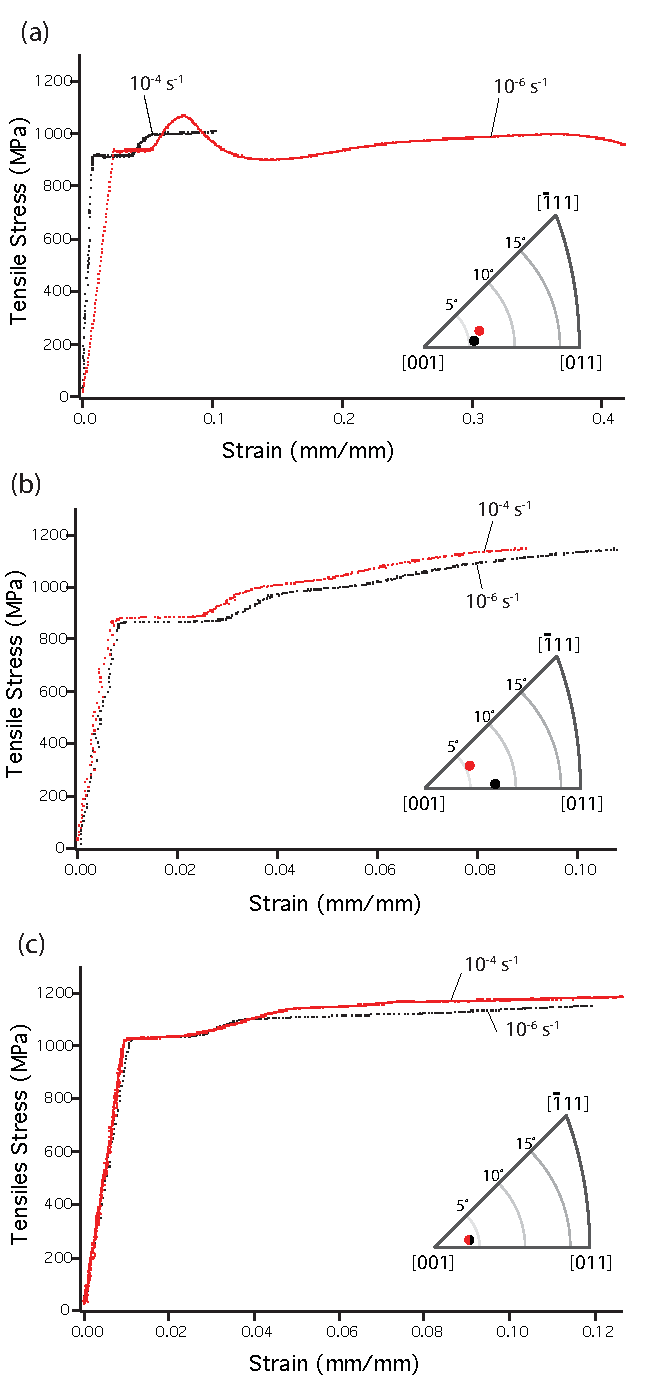
\includegraphics[width=\textwidth,height=\textheight,keepaspectratio]{Figures/Figure2_vert.pdf}
\caption{Tensile data obtained from (a) CMSX-4, (b) TMS-138A and (c) SRR-99, all tested at 750\,$^\circ$C to failure at two strain rates: 10$^{-4}$\,s$^{-1}$ and 10$^{-6}$\,s$^{-1}$. Neither }
\label{fig:138ASRR99_curves}
\end{figure}

Figure \ref{fig:x4_stressstrain} shows the stress-strain curves associated with tensile tests on specimens of CMSX-4 obtained tested to failure at 750$^{\circ}$C for three different strain rates,  $\dot{\epsilon}$: 10$^{-2}$\,s$^{-1}$ (the green curve), 10$^{-4}$\,s$^{-1}$ (the red curve) and 10$^{-6}$\,s$^{-1}$ (the blue curve). The specimen all had orientations within 10$^\circ$, as shown by the inverse pole figure in the top right of Figure \ref{fig:x4_stressstrain}. All curves show a linear progression up to around 950\,MPa. The curves then plateau for varying portions of strain. Beyond this point, the three curves exhibited different behaviours. The tensile curve run at 10$^{-2}$ increased in stress around 4\% strain to 1000\,MPa before plateauing again until 9\% strain, where the stress again increases at a gradual incline, before failure just before 15\% strain.\\
The tensile curve produced from the tensile test at 10$^{-4}$\,s$^{-1}$ maps a similar path to the tensile test at 10$^{-2}$\,s$^{-1}$, but after increasing in stress around 4\% strain to 1000\,MPa, the stress doesn't increase any further. Failure occurs in comparison at a much lower strain rate of 11.5\%.\\
The tensile curve from the tensile test at 10$^{-6}$\,s$^{-1}$ exhibited the shortest plateau; the stress remains at 950\,MPa to around 3\% strain before the stress drops and continues to do so down to 750\,MPa at around 8\% strain. After this, the stress rises again, at a slower rate, before failing around 23\% strain.
Further tests were run at the three different strain rates and interrupted at various points before failure. For the strain rate at 10$^{-2}$\,s$^{-1}$, another tensile test was run and interrupted at 3.3\% strain. Another tensile test was run at 10$^{-4}$\,s$^{-1}$ to 4.8\% strain. Three further tests were run at the  strain rate: 10$^{-6}\,s^{-1}$, interrupted at strains of  1.2\%, 2.7\% and 10.2\% respectively.
Since the tensile specimens showed varying degrees of orientation away from the $[001]$ direction, each of the test conditions were tested in groups of similar orientation to minimise the effect of orientation. These tests were interrupted at those specific strain levels where the curves run to failure exhibited discontinuities. The interrupted stress strain curves overlap consistently with tensile tests run to failure. The tensile curves associated with these interrupted tests can be found in the appendix. A third interrupted test was run to 10.2\% but the stress strain curve was not recorded due to instrument failure. The microstructure is shown in Figure \ref{fig:x4_stressstrain}d.\\
TEM foils were produced from these interrupted test specimens of CMSX-4 and imaged to understand the progression of the deformation structure. Figure \ref{fig:x4_stressstrain}a is a TEM micrograph imaged a couple of degrees tilt away from the [001] zone axis, with two-beam contrast g = (220). The tensile specimen was tested at a strain rate 10$^{-4}$\,s$^{-1}$, at 750\,$^\circ$C, interrupted at 3.3\% strain. Dislocations are present in both the $\gamma$ and $\gamma^\prime$ phases. The dislocations in the $\gamma^\prime$ precipitates have adopted various configurations. Figure \ref{fig:x4_stressstrain}b is TEM micrograph from a sample deformed at a higher strain rate 10$^{-2}$\,s$^{-1}$ also at 750\,$^\circ$C. It was interrupted at a slightly higher strain, 4.8\%. The dislocation structure is similar to that of Figure \ref{fig:x4_stressstrain}a, with dislocations present in $\gamma^\prime$ precipitates and $\gamma$ channels.\\
The TEM micrographs for interrupted specimens at the slowest strain rate, 10$^{-6}$\,s$^{-1}$ are shown in Figure \ref{fig:x4_stressstrain}(c-e). Interrupted at 1.2\% strain, the tensile specimen has reached a stress plateau. Dislocations are confined to distinct slip bands, with some areas of the microstructure free of any dislocations. At 2.7\% strain, stacking faults appear in the slip bands. Portions of the microstructure still remain free from dislocations. The stress continues to drop and the TEM micrograph interrupted at 10.2\% (Figure \ref{fig:x4_stressstrain}e) around the lowest stress shows these slip bands have widened to cover more of the microstructure.\\%A secondary slip system $<112>$\{111\} has become active
Tensile tests were also run for two further alloys: TMS-138A and SRR-99, across two strain rates: 10$^{-4}$\,s$^{-1}$ and 10$^{-6}$\,s$^{-1}$. The tensile curves are shown in Figure \ref{fig:138ASRR99_curves}. 
%1.2 \% strain is when the stress reaches its 750 MPa, the lowest value. The additional test interrupted at 2.5 \% was completed to see how the deformation features causing the drop in stress developed with further strain.
%In the slower strain rates, dislocations do not need to be generated as rapidly to accommodate the strain. Dislocations would therefore be expected to nucleate slowly confined to slip bands. This could also be due to the lower percentage of strain contained within the material as well as the orientation of the sample.\\
% Since the stacking faults appeared within the same activated slip system as the earlier test (LC1), this indicates that the drop not only coincides with the activation of additional slip system, but also the activation of another deformation mechanism (i.e. stacking fault shear). At this stage it is unclear which factor causes the drop in stress.
The respective orientations for each tensile specimen are shown on the inverse pole figure inset of Figures \ref{fig:x4_stressstrain} and \ref{fig:138ASRR99_curves}. Each of the test conditions were tested in groups of similar orientation to minimise the effect of mis-orientation.\\ %Please note that none of the orientations are expected to activate multiple slip systems.
%The deformation structures outlined above were all observed up to the yield point.
%1.2 \% strain is when the stress reaches its 750 MPa, the lowest value. The additional test interrupted at 2.5 \% was completed to see how the deformation features causing the drop in stress developed with further strain.
%At 1.2 $\%$ strain, the slip bands present in the interrupted microstructure at yield had become filled with stacking faults. Upon further deformation, By 2.5 $\%$ strain, these slip bands had widened and were close to completely filling the imaged area. This suggests that the preferred deformation mechanism causing the drop in stress is stacking fault shear.\\
%Strain stress curves at different strain rates at 750$^\circ$C. Interrupted tests (at yield and X strain) and associated microstructures ? general overview. All specimen are orientated along XXXX. 
%At yield ? microstructure ? starting point for the rest
%MSR ? dislocations in gamma ? higher density and gamma prime ? dipoles ? localized deformation in two slip system creating slip plane networks.
%HSR ? similar to MSR (to do: look more in detail ? deformation bands localisation).
%SSR ? slip bands on two slip systems. Mixture of interfacial dislocations and dipoles. Very localised slip bands 
%Talk about the trend ? slow strain ? more localised.

%Beyond yield ? at specific strain associated with features in the stress-strain curves.
%	MSR (@x1) ? greater intensity of the dislocation structure already established at yield. Activation of additional slip systems. Dipoles in multiples directions. Greater activity in the gamma channels.
%	MSR(@x2)  - same the previous structure observed in both MSR-yield and MSR-x1 with additional stacking faults going through gamma prime precipitates (? Attribution of the decrease in stress associated with the presence of stacking faults)
%	HSR ? Similar to MSR-yield and MSR-x1. 
%	SSR  (@y1) ? Dislocations bands filled with stacking faults as well as dislocation structure established and observed at yield in both already active slip systems. Therefore the additional strain is accommodated by the formation of stacking fault, which result in stress decrease.
%	SSR (@y2) ? activation of the both dislocations and stacking faults across the microstructure. Slip bands have widened significantly.
%Focus on the dislocation morphology
%(?Quick description of the dislocation structure present at yield across all the SR tests)
%Investigate stacking fault formation in MSR(@x2) and SSR(@y1), since less deformation and less SF to investigate in the SSR(@y1) so we choose to focus on this one, but we look (and show) at MSR(@x2) which show similar features.
To further investigate in detail the stacking faults observed in the Figure \ref{fig:x4_stressstrain}d and e, Laue back-reflection method was used to determine the primary slip system of the tensile specimens after tension. This allowed for precise sectioning of the specimen; first parallel and then perpendicular to the active slip system, on which the stacking faults were present. Conventional TEM imaging was performed on specimens cut parallel to the primary slip system, exposing the stacking faults within the plane and dislocations that bound such faults.\\
\begin{figure}
\centering
\includegraphics[width=\textwidth,keepaspectratio]{Figures/Figure3_twobeamconditionimagingaround111_v4.pdf}
\caption{STEM micrographs of the microstructure of [001] tensile specimen deformed at a strain rate of 10$^{-6}$\,s$^{-1}$ to 2.7\% strain, cut on the (1$\overline{1}$1) plane. All sub figures are taken over the same area of the sample. Starting at the centre, then working right and clockwise: (a) A schematic illustration of the dislocation structure, down the [1$\overline{1}$1] zone axis. (b) Two beam contrast, \textbf{g} = ($\overline{2}$02). (c) \textbf{g} = (11$\overline{1}$). (d) \textbf{g} = (022). (e) \textbf{g} = ($\overline{1}$11). (f) \textbf{g} = ($\overline{2}\overline{2}$0). (g) \textbf{g} = (111). Highlighted planes which are parallel to the electron beam are shown in inset of each subfigure.}
\label{fig:SF}
\end{figure}
Figure \ref{fig:SF} shows the microstructure of the tensile specimen deformed at a strain rate pf 10$^{-6}$\,s$^{-1}$ to 2.7\%, cut on the (1$\overline{1}$1) plane, the active slip system. In the middle, Figure \ref{fig:SF}a is a schematic illustration of the dislocation structure. It shows a stacking fault spread on the (1$\overline{1}$1) plane, bound by a total of six dislocation lines, four on one edge, two on the other, shearing a $\gamma^\prime$ precipitate. The dislocation are continuous, crossing both $\gamma^\prime$ precipitates and the $\gamma$-channels and seem to progress faster in the channels than the precipitates.\\The surrounding six images are STEM micrographs taken under six different two-beam conditions, at different degrees of of rotation away from the [1$\overline{1}$1] zone axis. The white arrows in each of the subfigures are the g-vectors, pointing in the direction of the respective reciprocal lattice planes. Through tilting the sample to varying degrees away from the [1$\overline{1}$1] zone axis, the red planes in the subfigure can be aligned parallel to the electron beam. Any dislocations on these planes would therefore have no impact on the transmission electron beam ($\textbf{g}$$\cdot$$\textbf{b}$=0) and appear invisible on the STEM micrograph under that respective two-beam imaging condition. By tilting the sample to the six different two-beam conditions of Figure \ref{fig:SF}, it is possible to deduce the Burgers vectors of the dislocations that bound the stacking fault.\\
The six dislocations are labelled 1-6. Starting with Figure \ref{fig:SF}b, all dislocations are not visible in this subfigure. The six dislocations are marked on a 3-point scale of visibility: i (invisible), w (weak, visible but not very strong) and v (visible). Going through each of the six micrographs, a visibility table is built up, as shown in Table \ref{tab:SF}. 
From the behaviour of the dislocations and the separation of these on the right hand side, it can be deduced that although these are contained in the same slip system they are actually located on different, parallel slip planes. A Burger vector analysis of the dislocations present reveals that these are of $[121](1\overline{1}1)$ type, although it is not possible to establish whether they are superpartial $\frac{a}{3}[121]$ or dissociated partials $\frac{a}{6}[121]$. Determining the direction of the Burgers vectors was challenging due to the presence of residual contrast from the faults that are produce in the $\gamma^\prime$ precipitate and interactions between the close spacing of the dislocations.\\
%The invisibility criteria associated with these dislocations is summarised in Table \ref{fig:SF}. However, the stacking faults influenced the adjacent dislocations' contrast and even from the best effort, it could only be deduced that the dislocations had a Burgers vector of [121]. Specific Burgers vectors could not be individually distinguished. The fact that the dislocations are closely spaced, influences the dislocation contrast. Which does not give a visibility criterion, which prevents the clear definition of the Burgers vector.
\begin{table}[bh]
	\caption{Table of visibility for the dislocations viewed down the $[1\overline{1}1]$ zone axis in Figure\,\ref{fig:SF}. '*' Figure\,\ref{fig:SF}(a) and (b) are not clear due to dislocation interactions and strain contrast.\hspace{\textwidth} i=\,invisible, w=\,weak, v=\,visible.}
    \centering
	\label{tab:SF}
	\resizebox{\textwidth}{!}{%
	\renewcommand{\arraystretch}{1.25}
	\begin{tabular}{l || cccccc | c|c}
	\rowcolor{Gray}
	\hline
Locations    & $[\overline{1}11]$ & $[11\overline{1}]$ & $[111]$ & $[\overline{2}\overline{2}0]$ & $[022]$ & $[\overline{2}02]$ & Burgers vector \\ \hline %\hline
number 1 & w* & v & v & v & v & i & $[121]$ \\ \hline
number 2 & v & v & i & v & v & i & $[121]$ \\ \hline
number 3 & i/w* & i/w* & v & v & v & i & $[121]$ \\ \hline
number 4 & i/w* & i/w* & w & v & v & i & $[121]$ \\ \hline
number 5 & v & v & v & v & v & i & $[121]$ \\ \hline
number 6 & v & v & v & v & v & i & $[121]$ \\ \hline
	\end{tabular}
	\renewcommand{\arraystretch}{1}
}
\end{table}
%\vspace*{-10pt}

\begin{figure}
    \centering
    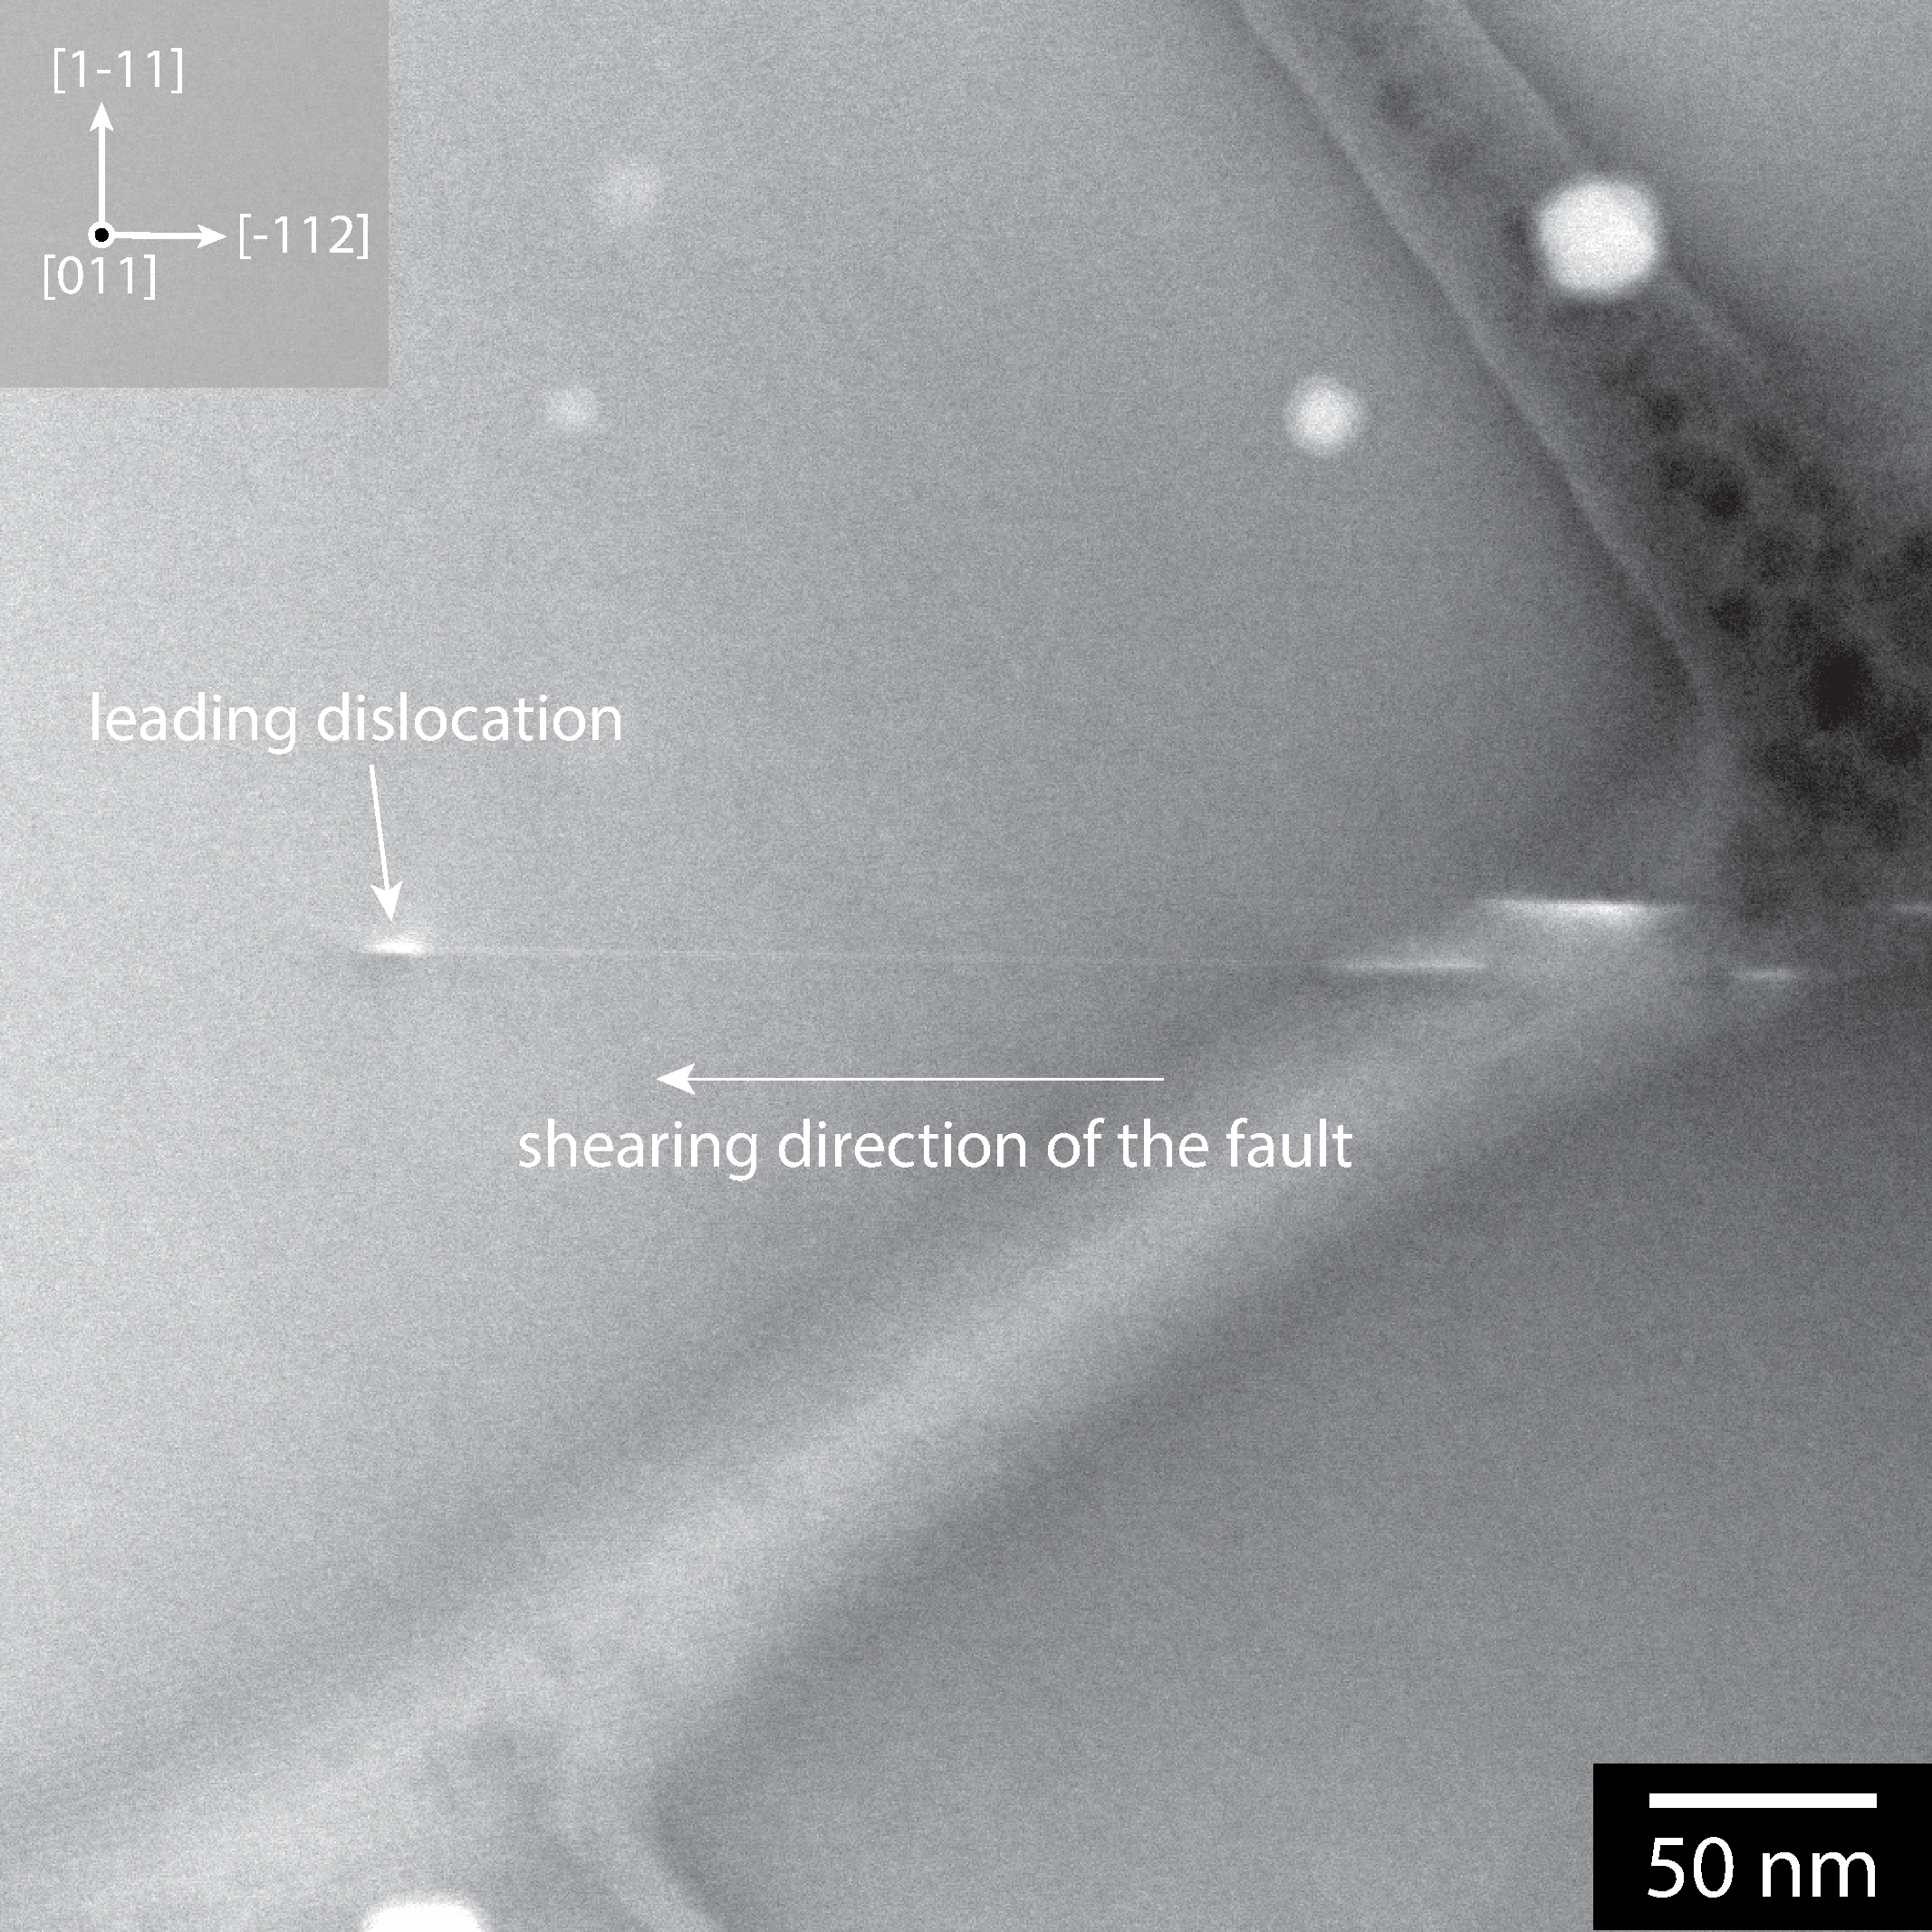
\includegraphics[width=\textwidth,height=\textheight,keepaspectratio]{Figures/142041.pdf}
    \caption{HAADF-STEM micrograph of a stacking fault imaged down the $[011]$ zone axis from a tensile specimen of CMSX-4, deformed at 750\,$^\circ$C at a strain rate of 10$^{-6}$\,s$^{-1}$ interrupt at 2.7\% strain. A stacking fault can be seen propagating from right to left, with the leading dislocations highlighted.}
    \label{fig:HAADFSTEM_SFshear}
\end{figure}

To more accurately establish the magnitude of the Burgers vectors of the dislocations, and in turn the stacking fault shearing mechanism, the sample was further cut on the (011) plane so that the Burgers vectors of the dislocations bound either side of a shearing stacking fault would have its maximum edge component perpendicular to the cut plane. Figure \ref{fig:HAADFSTEM_SFshear} shows a HAADF-STEM image of a stacking fault captured edge-on, down the $[10\overline{1}]$ zone axis. A fault can be seen propagating from right to left with the leading dislocation highlighted in the HAADF condition. Tertiary $\gamma^\prime$ precipitates in the $\gamma$-channel are also visible.
 The leading dislocation presents a high contrast compare to the background; the stacking fault can also be visualised by the presence of a faint line that runs from the leading dislocation to the $\gamma$/$\gamma^\prime$ interface where the contrast increases signalling the trailing dislocation is present.\\
 Lattice imaging of the leading dislocation was carried out and presented in Figure \ref{fig:haadfcos}a. The stacking fault's location corresponds to the region which has a slightly higher contrast to the background, although to highlight it further, a centre of symmetry analysis was performed from the processed image, and is presented in Figure \ref{fig:haadfcos}b. The imaged stacking fault is propagating from right to left. It shows a two-layered, intrinsic fault (SISF) terminating as a three-layered, constricted extrinsic fault (CESF-1), all within a $\gamma^\prime$ precipitate.\\
\begin{figure}
\includegraphics[width=\textwidth,height=\textheight,keepaspectratio]{Figures/HAADF_COS_v1.pdf}
\caption{(a) A low magnification HRSTEM image of a stacking fault from a tensile sample of CMSX-4 tested at 750\,$^\circ$C at a strain rate $\dot{\epsilon}$ = 10$^{-6}$\,s$^{-1}$, interrupted at 2.7\% strain. The sample has been cut on the (011) plane. The stacking fault is viewed edge on and can be seen in both the $\gamma^\prime$ precipitate and $\gamma$ channel. (b) The corresponding Centre of Symmetry (CoS) mapping with Burgers circuit shows a fault which is spread over two layers. (c) A schematic illustration of the hypothesised mechanism for the formation of the leading edge of the stacking fault.}
\label{fig:haadfcos}
\end{figure}
%In Nickel and Cobalt superalloys crept at high temperature, stacking fault formation has also been associated with the presence of chemical segregation. EDX and EELS maps were collected to establish the possible presence of chemical segregation at the stacking fault.

%The formation of the dislocation structure was imaged under WB2DF CTEM conditions in six conditions to determine the Burgers vectors of the dislocations and characterise the faults. The dislocations lie on (111) plane and adopt different configurations whether they are located in the $\gamma$ and $\gamma^\prime$ phases.

%HR STEM was conducted using an FEI Titan 3 STEM featuring a monochromator and a probe aberration corrector was used to perform the HAADF imaging. Figure \ref{fig:haadfcos} shows a \added[id=om, remark={not the raw image}] (raw) HR STEM image accompanied by the corresponding COS analysis reveals the presence a stacking fault shearing through a $\gamma^{\prime}$ precipitate.

%The HAADF images show stacking faults propagating through the $\gamma$ and $\gamma^{\prime}$ phases. Figure \ref{fig:haadfcos} is an example of a stacking fault terminating within the $\gamma^{\prime}$. 
The Burgers circuit traced around the fault segment requires a displacement vector of $b=\frac{a}{4}[121]$ in the observed plane. This is consistent with a dissociated pair of partials in the $\gamma^\prime$ of $\frac{a}{3}\langle 112\rangle$ and $\frac{a}{6}\langle 112\rangle$. The distance separating these two Shockley partials is approximately 13 lattice spacings. Taking $a_{\gamma^{\prime}}$ = 0.3627\,nm, the width of the fault is estimated to be 2.89\,nm. Since the stacking fault is bounded by partial dislocations with identical Burgers vectors, the equation below can be used to estimate its energy:
\begin{equation}
\gamma = K\frac{Gb^{2}}{2\pi d}
\end{equation}
Taking G = 105\,GPa and K = 1, the energy of the CESF-1 is 120\,mJ $m^{-2}$. This estimation is lower than the value 271\,mJ $m^{-2}$ predicted by the EAM model using Michin's potential but of similar value (137\,mJ $m^{-2}$) to that found empirically by Vorontsov et al.\cite{}\cite{}  The difference with Mishin's predicted value could be due to the chosen values of K, G, $a_{\gamma^{\prime}}$ and alloying effects. There is evidence of segregation of high Z elements to the fault, as will be shown by EDX spectra below. Furthermore, stacking fault energies are lower at elevated temperatures; the alloy was tested at 750\,$^\circ$C compared to -273\,$^\circ$C used in the model. The observed configuration shows the leading $\frac{a}{3}[121]$ superpartial dissociates into two identical $\frac{a}{6}[121]$ Shockley partials separated by a complex stacking fault lying on adjacent planes. This supports the idea that the stacking fault shear mechanism observed here is the same as the viscous shear mechanism of primary creep outlined by Kear et al.\cite{} and observed and predicted by Vorontsov et al.\cite{}.
\begin{figure}
    \centering
    \includegraphics[width=\textwidth,height=\textheight,keepaspectratio]{Figures/EDXmapsofSF_v1.pdf}
    \caption{EDX maps showing spatial distributions of the elements Cr, Co, Al, W and Ni, taken over two regions of the microstructure from a sample of CMSX-4 deformed at a strain rate of 10$^{-6}$\,s$^{-1}$ at 750\,$^\circ$C, interrupted at 2.7\% strain. (a) A STEM-HAADF micrograph imaged down the [011] zone axis, showing a stacking fault in a $\gamma^\prime$ precipitate. The EDX scans were taken from the front of the fault and a section midway along the fault, labelled as scan regions 'A' and 'B' respectively. (b) A HAADF image of the zoomed-in region 'A', (c)-(f) show the compositional EDX maps from region A for the elements Cr, Co, Al, W and Ni respectively. (g)-(l) show the compositional EDX maps for region B for elements Cr, Co, Al, W and Ni respectively.}
    \label{fig:edx_maps}
\end{figure}
\begin{figure}
    \centering
    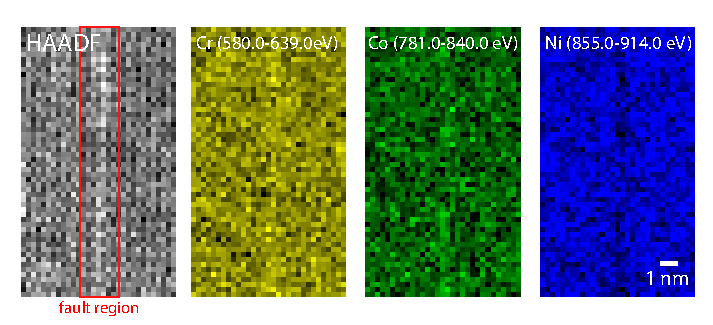
\includegraphics[width=\textwidth,height=\textheight,keepaspectratio]{Figures/EELSmap_v1.pdf}
    \caption{STEM-EELS mapping of composition in the vicinity of a stacking fault. (a) STEM-HAADF survey image of the stacking fault and adjacent area used for EELS mapping. (b-d) Compositional maps corresponding to Cr L$_{2,3}$, Co L$_{2,3}$ and Ni L$_{2,3}$ edges respectively.}
    \label{fig:EELS_maps}
\end{figure}
EDX maps were collected in an interval of 2.5 \%nm with drift correction in place to check for evidence of chemical variation at and around the stacking faults. An EDX map was acquired of the region in Figure \ref{fig:edx_overall} depicting a leading dislocation pair. Figure \ref{fig:edx_overall}a shows segregation of Cr and Co at the front-end of the fault. There is also an enrichment of W and Ta to the dislocation core though this is not as pronounced as the Cr and Co. Cr and Co segregation is also observed along the length of the fault (region B in Figure \ref{fig:edx_maps}). There is also a depletion of Al and Ni. Both effects occur along the length of the fault despite the HAADF image showing non-uniform brightness across the length of the fault. it is not clear whether W and Ta are segregating to or away from the fault. %as if the fault passing through picks up and drops off elements as it passes through the $\gamma^{\prime}$ precipitate.
In addition, above the fault is a trail of chemical depletion, perhaps from a previous fault. It is thought that this segregation might facilitate the passing of further dislocations since the local composition along the fault channel is already favourable.
EELS mapping was also conducted in a region containing the middle part of a stacking fault and the adjacent area. Compositional maps were taken corresponding to the Cr L$_{2,3}$, Co L$_{2,3}$ and Ni L$_{2,3}$ edges and are shown with the STEM-HAADF survey image in Figure \ref{fig:EELS_maps}. An enrichment of Cr and Co and a depletion of Ni along the fault is just about visible, though the segregation to the fault is not as pronounced as in the EDX images. The images nevertheless show segregation of Cr and Co occurs to a stacking fault in this sample.
%Shearing of the $\gamma^{\prime}$ precipitates by a/2$<112>$ dislocations distorts the $\gamma$/$\gamma^{\prime}$ interface, changing an appearance from linear to serrated in appearance (see Area 3, 132118 or 132313). 
%WB2DF CTEM to established burgers vectors and therefore dislocation reaction in the gamma and gamma prime. However, unable to get precise burgers vector magnitude, but burgers vectors direction could be established.  Truth table for one example (show figure).

%In Nickel and Cobalt superalloys crept at high temperature, stacking fault formation has been associated with the presence of chemical segregation which linked with macroscopic mechanical behavior (SFE decrease ? easier to dissociate and facilitate dislocation glide ? can lead to twin). Therefore a specimen oriented edge on (after careful work ? specify the orientation of the TEM specimen). Look at it on the OSIRIS. Find evidence of segregation at the SF.

%To further established the burger vectors of the dislocation inside the gamma prime precipitate, the Titan was used. EELS map was collected to support the result obtained from the OSIRIS.

%Segregation is removed after the passage of SFs.

% chemical diffusion, distances are predicted from ThermoCalc, are values reasonable and give plausible evidence of empirical observations?
% effect of composition?
% Calculate width of SFs and APB, estimate energies. Estimate diffusional distance from Thermocalc, compare against empirical data.

%literature value of SESF and SISF energies for TMS-138A.

%%%%%%%%%%%%
% Discussion
%%%%%%%%%%%%%
\section*{Discussion}
\subsection*{Formation of SESF Terminating in \texorpdfstring{$\gamma^\prime$}{Precipitate}}
%recognise that creep deformation has been mimicked in tensile deformation at slow strain rates%
The stress-strain curves and associated microstructural analysis show the formation of stacking faults is a strain-rate-dependent phenomenon. Figure \ref{fig:haadfcos} shows the front end of the fault features in Figure \ref{fig:SFshear} consists of a SISF terminating in a $\gamma^\prime$ precipitate, terminating in a two-layer CESF-1 type fault. The dissociation of the Shockley partials bounding this complex stacking fault is so small that it is not conclusive from the Burgers vector analysis of Figure \ref{fig:SF} in Table \ref{tab:SF}. However, the HAADF images and COS analysis of Figures \ref{fig:SFshear} and \ref{fig:haadfcos} show a two-layer CESF-1 terminating a superlattice intrinsic stacking fault (SISF).\\
This fault structure has been previously observed in samples deformed under primary creep at intermediate temperatures (750\,$^\circ$C). The structure of these dislocation ribbons has been extensive studied. These a$\langle112\rangle$ ribbons are dissociated into partial dislocations enclosing a low-energy superlattice intrinsic or extrinsic fault (SISF and SESF respectively) as shown in equation \ref{eq:SF}:
\begin{multline}
2 \times \frac{a}{2}[\overline{1}12] \rightarrow \frac{a}{6}[\overline{1}12] + \textbf{CESF-1} + \frac{a}{6}[\overline{1}12] + \textbf{SISF}\\
+ \frac{a}{6}[\overline{1}12] + \textbf{APB} + \frac{a}{6}[\overline{1}12] \\+ \textbf{SESF}
+ \frac{a}{6}[\overline{1}12] + \textbf{CISF} + \frac{a}{6}[\overline{1}12]
\label{eq:SF}
\end{multline}
where CISF is a complex intrinsic stacking fault and CESF-1 is a complex extrinsic stacking fault with high-energy bonding-violation on one side of the fault.\\
This full a$\langle112\rangle$ dislocation dissociation is rarely observed in a single $\gamma^\prime$ precipitate. Instead, to avoid the high-energy anti-phase boundary (APB) energy, the dislocation ribbon, either side of the APB, occupies adjacent precipitates where they are separated by perfect crystal in the $\gamma$ matrix. Due to the very high fault energy of both complex faults, the two $\frac{a}{6}\langle112\rangle$ Shockley partials are very closely separated by complex stacking faults and under insufficient resolution are observed as one $\frac{a}{3}\langle112\rangle$ superpartial.\cite{}\\
The fault in Figure \ref{fig:SFshear} and \ref{fig:haadfcos}b consists of a $\frac{a}{6}\langle112\rangle$ zonal partial ($\delta$C + $\delta$A, which is equivalent to B$\delta$ spread on two adjacent (111) planes), followed by a $\delta$B partial on a single (111) plane and finally a two-layer fault consisting of an APB over an SISF.\\
Figure \ref{fig:CESF_mech} shows the sequence of events proposed to form the leading extrinsic fault. It starts with two dislocations reaching adjacent planes (Figure \ref{fig:CESF_mech}a). The leading partials of the two $\gamma$ lattice dislocations then enter to form a CESF followed by one of the trailing partials (\ref{fig:CESF_mech}b); and the fourth partial remains at the interface whilst a reordering process produces an SISF in the $\gamma^\prime$ (\ref{fig:CESF_mech}c). This mechanism would explain why this phenomenon was not observed in TMS-138A, where the interfacial dislocations have restricted climb.\\
\begin{figure}
\centering
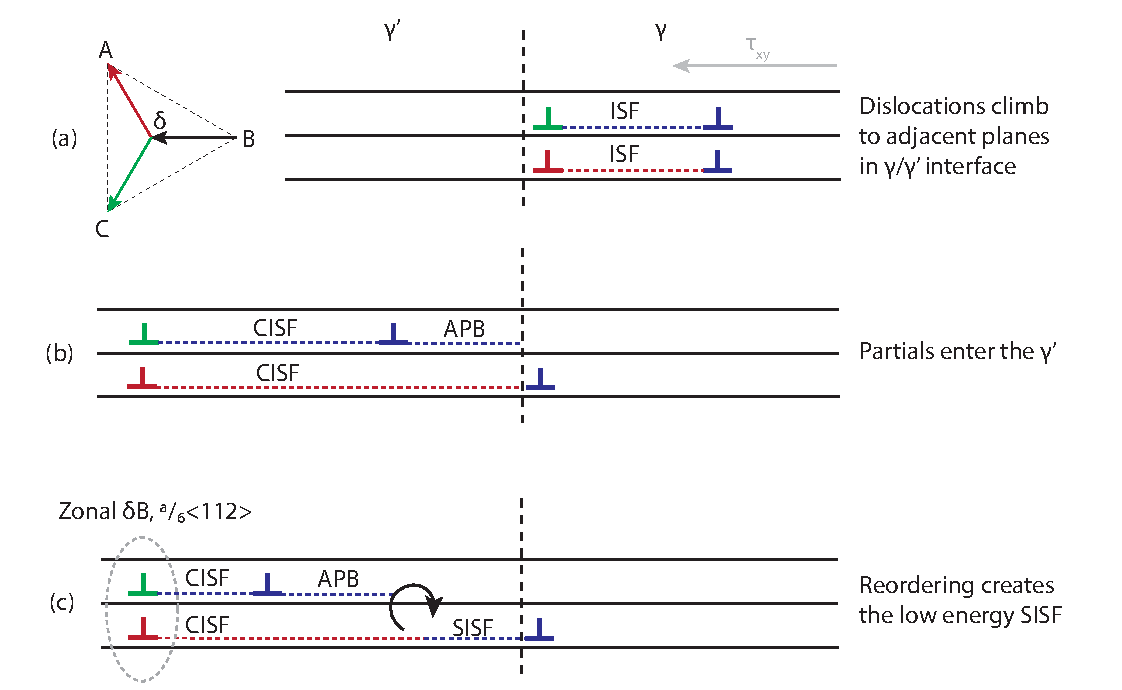
\includegraphics[width=\linewidth, keepaspectratio]{Figures/CESF_mech2_schem.pdf}
\caption{{Proposed mechanism for the f}ormation of a SISF from two dislocations climbing in the $\gamma$/$\gamma^\prime$ interface. The arrow represents reordering.}
\label{fig:CESF_mech}
\end{figure}
The CESF-1 fault forms by the dipole displacement occurring at the second, trailing partial $\frac{a}{6}\langle112\rangle$. Kear et al. suggested such displacements can be achieved through atomic shuffling at the partial dislocations bounding the extrinsic fault. Such mechanisms would be favoured at elevated temperatures and lower strain rates, hence they are observed during creep. The lowering of the strain rate during tensile deformation would allow sufficient time for vacancy migration to occur, facilitating the shearing of $\gamma^\prime$ precipitates by stacking faults.\\
%The alternate mechanism involves the climb of two $\frac{a}{2}\langle112\rangle$ dislocations in the $\gamma$ channels with Burgers vectors at $60^\circ$.\cite{} The SISF would form when the two dislocations reach adjacent planes. Through a process of reordering, an SISF is then formed within the $\gamma^{\prime}$.\cite{}\\
%Kear and co-workers defined a viscous slip mechanism for stacking fault shear during primary creep. An SISF-SESF pair is created, but they are part of an a$\langle112\rangle$ dislocation that originate on one glide plane. The complete stacking fault ribbon consists of two pairs of $\frac{a}{6}\langle112\rangle$ and $\frac{a}{6}\langle112\rangle$ partials.
%A complete a$\langle$112$\rangle$ ribbon requires four $\frac{a}{2}\langle110\rangle$ matrix dislocations to form. Once in the $\gamma^{\prime}$ phase, the leading and trailing $\frac{a}{2}\langle110\rangle$ pairs dissociate into partial dislocations bounding an SISF and an SESF respectively. Assuming the applied stress is sufficiently high, the $\frac{a}{3}\langle112\rangle$ superpartial will be able to penetrate into the $\gamma^{\prime}$ precipitate. As it propagates, it leaves behind a SISF, and the trailing $\frac{a}{6}\langle112\rangle$ partial is left pinned at the $\gamma$/$\gamma^{\prime}$ interface. The $\frac{a}{6}\langle112\rangle$ is pinned at the interface because of the APB that would be created if it were to enter the precipitate. The trailing $\frac{a}{2}\langle110\rangle$ pair can dissociate to give an $\frac{a}{6}\langle112\rangle$ and $\frac{a}{3}\langle112\rangle$ pair of partial dislocations. If this trailing $\frac{a}{2}\langle110\rangle$ arrives at the interface, the dissociate $\frac{a}{6}\langle112\rangle$ and the trailing $\frac{a}{6}\langle112\rangle$ on the interface can enter the $\gamma^{\prime}$ separated by a small APB region. The pair leave behind a lower energy SESF. Finally the trailing $\frac{a}{3}\langle112\rangle$ dislocation enters the precipitate to clear the planar defects, leaving a perfect crystal. This process is given by the equation:
%Since a certain amount of time must pass for two dislocations of appropriate Burgers vector to meet at the $\gamma$/$\gamma^{\prime}$ interface to initiate the second shearing mechanism, it could be the rate determining step. The tensile test run at 0.06 mm/min transitioned from APB shear on two slip systems to stacking fault shear at x\% strain. Figure \ref{} shows the two slip systems active filled with dislocations mainly in the $\gamma$ matrix and stacking faults sharing $\gamma^{\prime}$. The Burgers vector visibility analysis showed a high majority of the dislocations have the same Burgers vector, $\frac{a}{2}\langle110\rangle$. It is difficult to discern whether interaction of the two slip systems could produce the appropriate dislocations to cause stacking fault shear. A plot of stress vs. time shows the drop in stress that corresponds to stacking fault shear occurs earlier than for the slowest strain rate 0.006 mm/min.
%how to transition to talk about climb shuffling?
\subsection*{Elemental Segregation at the Fault}
It is hypothesised that the local compositional changes from enrichment of Cr and Co and depletion of Ni and Al to the fault are required to lower the fault energies that are precursors to the SISFs and SESFs.\cite{} This is supported by the different segregation environments at the front of the fault (region A) compared to along its length (region B), namely the lack of depletion of Al and Ni and enrichment of W and Ta. Viswanathan et al. have shown similar compositional variation exists at SISFs created in the $\gamma^{\prime}$ precipitates for CMSX-4.\cite{} To achieve such compositional variations, they propose diffusion occurs along the cores of the partial dislocations and reordering adjacent to the fault. The lack of evidence of a compositional depletion zone adjacent to the fault disagrees with this mechanism. Furthermore, if diffusion was occurring and rate controlling along the length of the leading dislocation line, the segments closer to the $\gamma$ channels would have progressed the most through the precipitate, which is the opposite of the case observed in Figure \ref{fig:SF}.\\
An alternative mechanism is hereby proposed where the propagating fault is able to pick up segregating elements from neighbouring pockets of $\gamma$-former within the $\gamma^{\prime}$ precipitate. The EDX maps show a lack of uniform composition within the $\gamma^{\prime}$ precipitate, and it is these pockets of $\gamma$-former from which the fault can pick up and drop off elements to stabilise the propagating fault. The compositional profiles perpendicular to the fault show a 2 at.\% increase in Cr and Co, and a subtle decrease for Al. It is hypothesised that these compositional differences are small enough that it should be possible for elements to readily diffuse to and from the fault from these pockets of $\gamma$-former.\\
Vorontsov et al. have shown that both SISF and SESF faults show higher HAADF image intensity in CMSX-4, indicating diffusion-mediated segregation may be an essential process that controls shearing of the $\gamma^{\prime}$ precipitates at intermediate temperatures.\cite{}\\
DICTRA simulations were conducted on a six component alloy to understand whether bulk diffusion would be plausible within the time frame of SF shear. The macroscopic strain rate can be related to the dislocation velocity by Orowan's equation (Equation \ref{eqn:orowan}).
\begin{equation}
\dot{\epsilon} = \frac{1}{M}b\rho_{m}v
\label{eqn:orowan}
\end{equation}
M is the inverse Schmid factor. The dislocation velocity calculated here, $v$, corresponds to a complex dislocation network at steady-state and is regarded as the effective average velocity of mobile dislocations, as opposed to a single gliding dislocation. The density $\rho_{m}$ has been approximated using the Taylor model $\rho_{m}=(\frac{\tau}{\alpha Gb})^2$ where $\alpha$ is a constant, taken to be 0.3.\citep{} It has been shown above that the dislocations controlling plastic deformation at the slowest strain rate are of the type $\frac{a}{3}$$\langle112\rangle$$ \{111\}$. A Schmid factor of 0.4173 was used. The time-averaged mobile dislocation velocity can now be estimated using:
\begin{equation}
v = \frac{\dot{\epsilon}M}{b}\Big( \frac{\sigma}{M\alpha Gb} \Big) ^{-2}
\label{eqn:dislv}
\end{equation}
The flow stress $\sigma$ was taken to be the lowest value of tensile stress 750\,MPa. It is assumed this flow stress is the below the threshold stress to cause shearing through dipoles and therefore only stacking fault shear is occurring. A dislocation velocity was estimated at 2 nm$s^{-1}$.\\
It remains unclear whether the formation of stacking faults within a $\gamma^\prime$ precipitate is kinetically favourable, assisted by an adjacent region of $\gamma$-former elements that can stabilise the $\gamma^\prime$-stacking fault interface. To test this hypothesis, the time taken for elements to diffuse to a stacking fault through the precipitate bulk was simulated using \textit{Dictra}. Only the six main alloying elements were considered, as the inclusion of the other elements (in particular rhenium) slowed the calculation to an unfeasible extent.\\
The resulting composition profiles for four different calculation times are shown in Figure \ref{fig:dictra}: black (the initial composition profile), red (after 1E-9 seconds), blue (after 0.1 seconds) and purple (after 1 second). The projected interface location is marked above the composition profiles, in the colour corresponding to the time step. Only simulations for Co and Al are shown. Because it is only a six-component system, the W and Ta are not representative of how they would diffuse in a complete 10-component alloy system like CMSX-4 and were ignored as artefacts.\\
For the calculation of this segregation process, it was assumed that a pocket of $\gamma$-former elements was positioned 100\,nm away from the stacking fault. Upon running the simulation, these $\gamma$-former elements would diffuse through the bulk towards the stacking fault to stabilise it.
The four composition profiles show the element concentration of cobalt (top) and aluminium (bottom) in weight percent. While cobalt and tungsten partitions to the $\gamma$-phase, aluminium and tantalum  partition to the $\gamma^\prime$ phase.\cite{} As a result, the composition profiles either side of the $\gamma^\prime$-phase and stacking fault interface differs accordingly.\\
The composition profiles indicate the level of mobility of the respective elements through the precipitate. Aluminium has the fastest diffusion rate, and as a result shows nearly homogeneous concentration profile after 1e-9 seconds. Cobalt is slightly slower and therefore only reaches a homogeneous concentration profile after one second. The diffusion rate and profile of chromium is very similar to the result shown for colbalt and not shown in Figure \ref{fig:dictra}.
The results from the \textit{Dictra} simulations show that for a pocket of $\gamma$-former 100\,nm away from the fault, the elements are able to diffuse through the bulk, causing an enrichment of colbalt and chromium and a depletion of aluminium within a stacking fault. The segregation can occurs over an extremely short period of time (t = $1\times 10^{-9}s$). This shows that the segregation of cobalt and chromium and depletion of aluminium in the EDX maps (Figure \ref{fig:edx_maps}) is kinetically possible. Especially since the elements will diffuse over much shorter distances than 100\,nm with many $\gamma$-former pockets located adjacent to the fault.\\
\begin{figure}
    \centering
    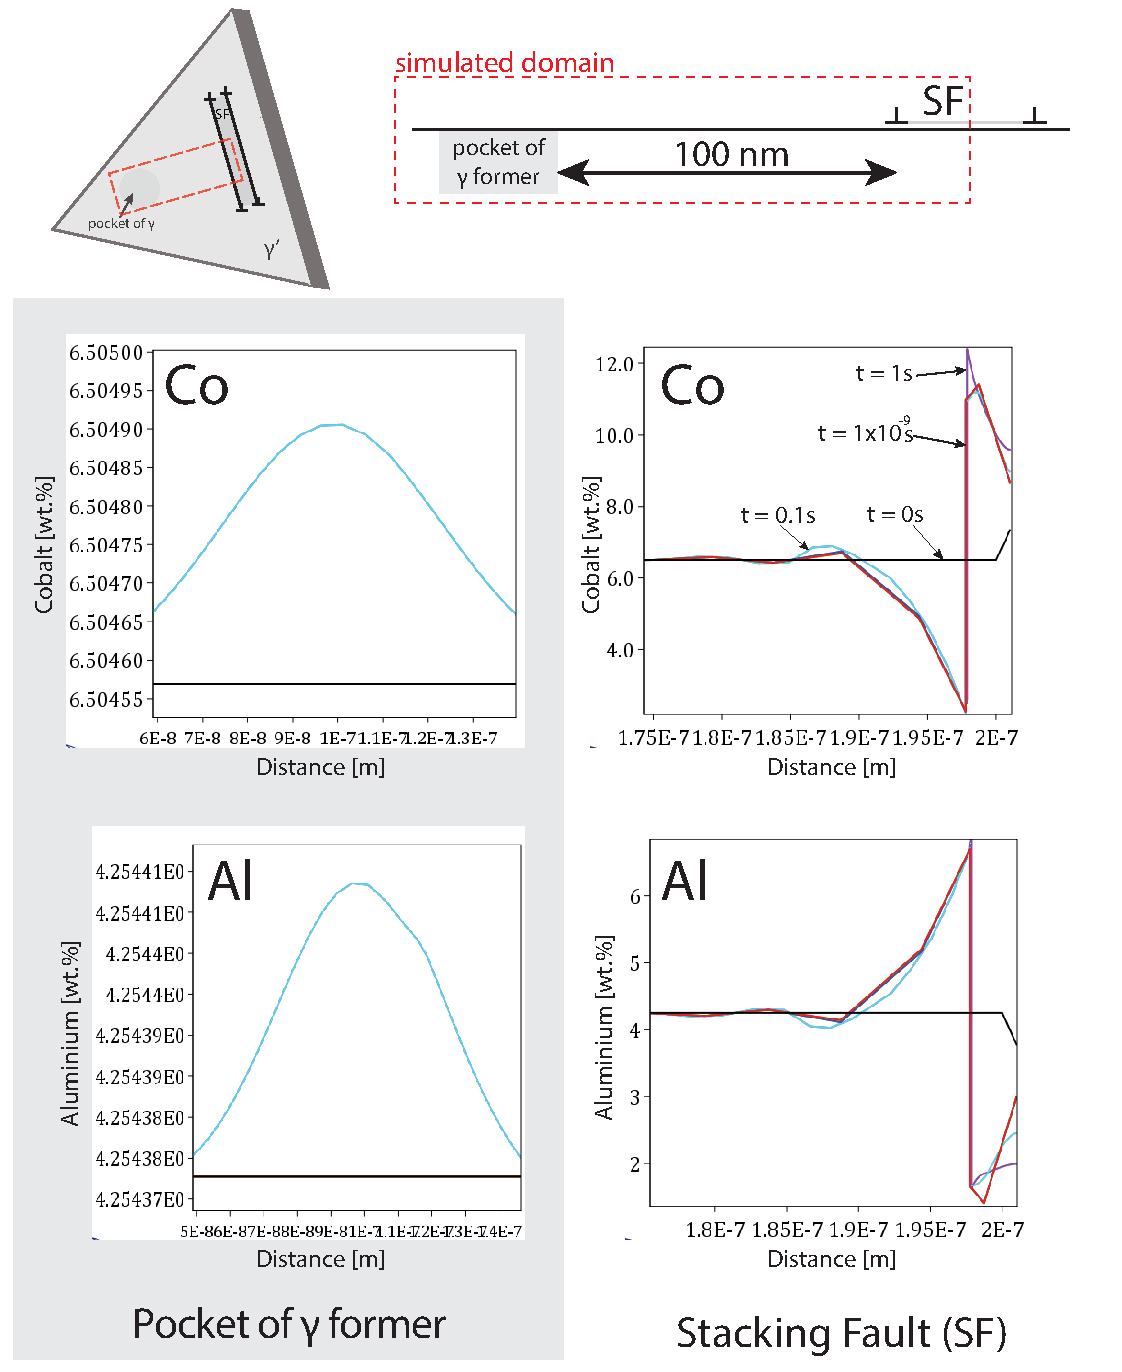
\includegraphics[width=\textwidth,keepaspectratio]{Figures/dictra_simul_1.pdf}
    \caption{Composition profiles from a \textit{Dictra} element distribution simulation of the diffusion of $\gamma$-former elements to a stacking fault composition region using only six major alloying elements of CMSX-4. The composition profiles for the elements cobalt (top) and aluminium (bottom) are shown for the pocket of $\gamma$ former (top left and bottom left) and at the $\gamma^\prime$-stacking fault interface (top right and bottom right). The composition profiles for different calculation times are plotted in black (initial profile), red (1E-9 seconds), blue (0.1 seconds) and purple (1 second).}
    \label{fig:dictra}
\end{figure}
%The homogenisation heat treatment undertaken by these specimens prior to machining and testing may also be important. Smaller $\gamma^{\prime}$ precipitates would find it easier for the $\gamma$ to diffuse out of the $\gamma^{\prime}$ precipitate. Without these $\gamma$ pockets, stacking faults would be unstable and not form. If the threshold stress were high enough, deformation would proceed by APB shearing and the stress drop would not be observed. It has been shown for CMSX-4 that specimens with smaller precipitates perform worse in creep.\cite{Tabrizi2015Auth}\\
%In both cases, it is only energetically favourable if the two layer APB/SISF configuration can transform rapidly into a single-layer SISF as the $\frac{a}{3}\langle112\rangle$ propagates through the precipitate. Kear et al. suggested a vacancy-mediated reordering process or via cooperative shear and reordering of the two-layer CSF. The rate of this reordering process
%No segregation was observed within or around the dipoles, which precede stacking faults. This is evidence that the stacking faults do not originate from dipoles.
%The stacking faults might also be a product of dislocations from two slip systems. However, stacking fault shearing is the deformation mechanism as soon as the specimen yields at the slowest strain rate. The time spent in the elastic regime probably allows sufficient diffusion to occur and the adoption of atomic configurations at the $\gamma$/$\gamma^{\prime}$ for SF shear.
% recognised mechanism of primary creep
%theory 1: SFs need a minimum threshold level of Co/Cr to form%
The segregation of Chromium and Cobalt to the fault suggests that a minimum threshold level of these two elements is required to form stacking faults. If there is insufficient Chromium or Cobalt, then the partial dislocations entering into $\gamma^{\prime}$ precipitates cannot be stabilised, preventing SF shear. Chromium and Cobalt preferentially partition to the $\gamma$ matrix phase.\cite{jarrett1982effects,tien1982effects,oni2016atom,llewelyn2017effect} As the precipitates form upon homogenisation, the supersaturated Cobalt and Chromium are rejected out into the matrix phase. This process continues upon further ageing. Therefore the heat treatment cycles which a superalloy is subject to prior to service is important. If the heat treatment cycles are not long or hot enough to allow appropriate amounts of Cr and Co to partition to the matrix, there will be a deficit within the vicinity of a partial wanting to shear the $\gamma^{\prime}$ precipitate, preventing the local chemistry required to stabilise it. This theory also extends to alloys with lower levels of Chromium and Cobalt. This would explain why no SF shear was observed in tensile tests at either strain rates for TMS-138A (see Figure \ref{fig:138ASRR99_curves}(b)). Compared to CMSX-4, the composition of TMS-138A is depleted in chromium and cobalt. Chromium and cobalt partition to the $\gamma$ phase, but the reduced quantity available in the alloy may result in a longer diffusion time, inhibiting stacking fault formation. Similar quantities of aluminium and Tungsten between the two alloys suggest they do not affect the rate of stacking fault formation.\\
Tensile tests were also performed on the first-generation superalloy, SRR-99 at the two different stain rates. The stress-strain curves are shown in Figure \ref{fig:138ASRR99_curves}(c). The curves showed no drop in stress. This alloy was tested because it is a high diffusion alloy. Therefore it would be expected that the dipole displacement that requires vacancy diffusion would be easier, facilitating stacking fault shear. Comparing the compositions of SRR99 and CMSX-4, SRR99 has a lower Cr and Co content. If there are insufficient levels to diffuse to the fault as it propagates, the stacking fault cannot form even if dipole displacement is easily achieved.\\

%\begin{figure}
%\includegraphics[width=\textwidth,height=\textheight,keepaspectratio]{SRR99.pdf}
%\caption{Stress strain curves obtained from tensile tests of SRR99 at two different strain rates: $\dot{\epsilon} = 10^{-6}\,s^{-1}$ and $\dot{\epsilon} = 10^{-4}\,s^{-1}$. Neither test showed a drop in flow stress.}
%\label{fig:srr99}
%\end{figure}

%Energies of SESF and SISF are being lowered by the local compositional change%

%theory 2: SF is a site of diffusion, becomes a time-dependent phenomenon%

%theory 3: Dislocation traps y-formers in its strain field and displaces y? formers when shearing y?%
In addition to diffusion, the EDX maps reveal the presence of tungsten and tantalum at the shearing dislocation's core. The diffusion distance is limited for tungsten and tantalum due to their slightly larger size. It is thought that tungsten and tantalum stabilise the dislocation core, getting trapped in its strain field, and displace $\gamma^{\prime}$-former elements during the shearing process. The introduction of tungsten and tantalum means aluminium and nickel need to be removed to balance the average atomic number, accounting for the depletion of aluminium and nickel within the fault. Furthermore, nickel and aluminium are depleted because they do not contribute towards stabilising the stacking fault and thus get pushed out of the dislocation strain field.\\
%dismiss theory 4: conversion to DO19 and DO24%
Titus et al. and Smith et al. proposed a local phase transformation from L1$_{2}$ to DO$_{19}$ and DO$_{24}$ for Co- and Ni-based superalloys respectively.\citep{} The local regions around the SESFs were also enriched with cobalt, chromium and molybdenum, and depleted in $\gamma^{\prime}$ formers Al, Ti, Ta and W.\\
It was hypothesised that the presence of cobalt and chromium at the tip of the fault lowers the CSF energy trailing the first Shockley partial, as well as the two layer CSF trailing the passage of the second Shockley partial. HAADF-STEM imaging showed ordered contrast along the SESFs consistent with a displacive-diffusive phase transformation from faulted $\gamma^{\prime}$ to the DO$_{24}$ structure ($\nu$ phase). However such a transformation would be permanent, which is not the case in the HAADF images above. Above the fault in figure \ref{fig:SFshear} shows the trace left by another stacking fault having passed through the $\gamma^{\prime}$. Though a faint outline may be visible on the HAADF image, the COS image shows the fault has disappeared along with any accompanying atomic displacement suggesting the segregation is also only temporary.\\
% effect of orientation
For orientations near [001], slip is available on any of the four $\langle$112$\rangle${111} slip systems. It has been shown that there exists a very strong orientation dependence of creep strength in Mar-M200.\cite{COPLEY197287} This dependence showed significant correlation with the Schmid factors of the active slip systems.
Creep strength was also investigated by MacKay and Maier on single crystal specimen of Mar-M247 deformed at 774\,$^\circ$C and 724\,MPa.\cite{MacKay:1982gd} The degree of misorientation away from the [001] tensile axis was shown to have a major influence on the stress rupture life.
%talk about Schmid factors, interaction of two slip systems entangling dislocations, current dislocations in slip bands prior to SFs forming


%This indicate that creep properties can be assess through careful tensile tests.

%What about the influence of the alloy composition (APB - ?.)

%(? Why does it happen later in MSR? ? associated with diffusion increased due to increase dislocation density or time depend or dislocation
%Tensile tests were also run at the strain rate $\dot{\epsilon}$ = $10^{-5}s^{-1}$. The stress strain curve is shown below in Figure \ref{fig:int}. The tensile stress is plotted against engineering strain because the extensometer used to measure strain slipped off the sample midway through the test run to failure. The curve initially follows the trend of standard single crystal deformation, up to $\epsilon_{eng}$ = 10.6\,\%, upon which a stress drop was observed. This stress drop ($\textasciitilde$ 200\,MPa) was similar magnitude to that which observed during tensile testing conducted at $\dot{\epsilon}$ = $10^{-6}s^{-1}$.
%Further tensile tests were run at $\dot{\epsilon}$ = $10^{-5}s^{-1}$ and interrupted at $\epsilon_{eng}$ = 0.05\,\% and 0.28\,\% respectively. The interrupted stress strain curves show consistent trends with the tensile test run to failure. Only in the test to failure does the stress drop below the yield stress. If the yield stress is above the threshold stress for both SF and APB shearing, deformation would be expected to continue with these two mechanisms in tandem.
%The microstructures for the interrupted tests are shown in Figure \ref{}. At the interruption before the drop in stress, as before dipoles are visible in the $\gamma^\prime$ precipitates and dislocations within both the horizontal and vertical $\gamma$ channels. Upon the drop in stress, stacking faults appear in the microstructure further supporting the hypothesis that stacking fault shearing causes the drop in stress.
%The easy glide portion of the stress strain curve for the tensile test at $\dot{\epsilon} = 10^{-6}\,s^{-1}$ is short and would suggest no secondary slip system is activated before the drop in stress. However, the stress strain curves featured in Figure \ref{fig:int} suggest secondary slip systems can be active prior to stacking faults appearing. A Burgers vector analysis was done around the [001] zone axis on the tensile specimen interrupted shortly after the drop in stress occurred. Four two-beam conditions were imaged which are shown in Figure \ref{fig:int}.
%The dislocations within the slip bands become invisible in the $g_{020}$ condition, suggesting they are all of the same Burgers vector, $b =  \frac{a}{2}[101]$. There are two conditions for which the stacking faults are invisible; the stacking faults contained within the horizontal slip band disappear in the $g_{\overline{2}20}$ condition, while the stacking faults in the vertical slip bands disappear in the $g_{220}$ condition. This would mean the stacking faults are bound by $\frac{a}{6}[112]$ and $\frac{a}{6}[\overline{1}1\overline{2}]$ partials, gliding on $(\overline{1}\overline{1}1)$ and $(1\overline{1}\overline{1})$ slip planes respectively.

%\begin{figure}
%\includegraphics[width=\textwidth, height=\textheight, %keepaspectratio]{Figures/200cx_overview_v2.pdf}
%\label{fig:int}
%\caption{TEM micrographs of the microstructure of [001] tensile %specimen deformed at a strain rate of 10$^{-5}$\,s$^{-1}$ at %750$^\circ$ interrupted at X\% strain, cut on the (001) plane, %perpendicular to the tensile direction. (a) Two beam contrast, %\textbf{g} = (200). (b) \textbf{g} = ($\overline{2}$20). (c) %\textbf{g} = (020). (d) \textbf{g} = (220). Highlighted planes %are shown in inset of each subfigure.}
%\end{figure}
\subsection*{Transition between APB and SF shearing}
The strain rate is related to the dislocation density by Equation \ref{eq:strainratedensity}, where $\rho$ is the dislocation density, $b$ is the Burgers vector of the dislocations and $v$ is the average velocity of the dislocations. Since there are two different processes by which dislocations can shear precipitates, Equation \ref{eq:strainratedensity} can be modified to Equation \ref{eq:sfandapb}.
\begin{equation}
\dot{\epsilon}=\rho bv
\label{eq:strainratedensity}
\end{equation}
\begin{equation}
\dot{\epsilon}=\rho_{APB}b_{APB}v_{APB} + \rho_{SF}b_{SF}v_{SF}
\label{eq:sfandapb}
\end{equation}
The threshold stress required for APB shearing is higher and this component will dominate at high strain rates and low temperatures. The stacking fault shear portion of the expression will be favoured at slow strain rates and high temperatures. In the slowest strain rate test ($\dot{\epsilon}=10^{-6}\,s^{-1}$), during the elastic region of the curve, dislocations are packing into the $\gamma$ channels. Upon yield, those dislocations pinned up against the $\gamma$/$\gamma^\prime$ interface will enter into precipitates. The strain rate is sufficiently slow that the atomic shuffling and segregation required to form stacking faults can occur. In addition, the temperature is high enough and the dislocations at the matrix/precipitate interfaces are correctly oriented for SF shear to occur. Because the threshold stress is propagate a stacking fault through the precipitate is lower than the yield stress (500\,MPa)\cite{}, once a proportion of the precipitates are shearing by stacking faults, the stress begins to drop. As strain in the sample increases, more dislocations will continue to shear by the formation of stacking fault ribbons until the majority of the dislocations are shearing by this method. This is reflected macroscopically in the stress strain curve by a drop in stress. This stress drop will continue until a high majority of the precipitates are filled with stacking faults which corresponds to the lowest stress. Finally, as these dislocation features begin to entangle, gradual work hardening occurs until failure.\\
%For the tensile test conducted at $\dot{\epsilon}=10^{-5}\,s^{-1}$, the stress-drop was only observed after a significant amount of work hardening after yield. Because stacking fault shear is a time-dependant phenomenon, only upon passing of an amount of time corresponding to this amount of stain (~15\,\%), is the relative orientations of the dislocations correct.\\
%Stress strain curves from tensile tests run at the same slow strain rates for different orientations are shown in Figure \ref{fig:138A_stressstrain}. The stress drop observed previously was not observed. It is thought that the initial orientations of these samples is such that the $\{111\}\langle112\rangle$ slip system, necessary for stacking fault shear, never becomes active.

%%%%%%%%%%%%
% Conclusions - needs strengthening
%%%%%%%%%%%%%
\section*{Conclusions}
Creep deformation by stacking fault shear can be induced in slow strain rate tensile tests. This phenomenon is only apparent for strain rates slower than $\dot{\epsilon}$ = 10$^{-5}$\,s$^{-1}$. This is associated with a drop in the flow stress after the yield point. Microstructural observations show the presence of stacking faults after this drop in stress. The deformation mechanism is analogous to viscous slip observed in primary creep. EDX and EELS maps of these stacking faults showed segregation of Cr and Co and depletion of Al and Ni at the fault. This segregation suggests stacking faults act as sites of diffusion and the shearing mechanism is a time-dependent phenomenon. The elements are able to diffuse to and from the fault through bulk diffusion in the $\gamma^{\prime}$ precipitates. Pockets of $\gamma$-former elements adjacent to the fault, visible through EDX scans, act as sites from which elements can diffuse to stabilise the fault. The formation of stacking faults and pseudo-creep deformation mechanisms is orientation dependent.
%Creep deformation by stacking fault shear can be induced in tensile tests, although a slow strain rate is required. This is associated with a drop in the flow stress after the yield point. Microstructure observations show the presence of stacking faults after this drop in stress. The deformation mechanism is analogous to viscous slip observed in primary creep. EDX and EELS maps of these stacking faults showed segregation of Cr and Co and depletion of Al and Ni at the fault.This segregation means stacking faults act as sites of diffusion and the shearing mechanism is a time-dependent phenomenon. The elements are able to diffuse to and to and from the fault through bulk diffusion in the $\gamma^{\prime}$ precipitates. Pockets of $\gamma$-former elements adjacent to the fault, visible through EDX scans, act as sites from which elements can diffuse to stabilise the fault. Orientation needs to be carefully controlled because this affects whether shearing by stacking faults occurs.

%\begin{appendix}

%\begin{table}[htbp]
%\centering
%	\caption{Orientation of all samples tested}
%    \begin{tabular}{c c c c c c c c}
%Sample & $\gamma$ & $\delta$ & $\theta$ & $\kappa$ & $\alpha$ & %$\rho$ & $\omega$ \\
%HSR1 (X409)& 3.6 & -3.7 & 5.2 & 58.9 & 58.9 & 13.3 & 315.5\\
%HSR2 & -7.6 & -1.4 & 7.7 & 1.5 & 1.7 & 12.2 & 79.4\\
%MSR1 & 3.9 & 0.3 & 3.9 & 10 & 10 & 13.7 & 266.3\\
%MSR2 & 1.3 & 6.2 & 6.4 & 29.5 & 29.4 & 17.5 & 192\\
%SSR1 & 3.6 & 4.6 & 5.8 & 13.6 & 13.9 & 24.2 & 218\\
%SSR2 &-2 & 5 & 5.4 & 0.5 & 0.3 & 21.7 & 158.7\\
%SSR3 & 1.5 & 5.4 & 5.6 & 0.5 & 0.3 & 21.7 & 158.7\\
%SSR4 & 5.6 & 0.3 & 5.6 & 80.7 & 80.7 & 6.7 & 267.4\\
%\label{tab:orient}
%\end{tabular}
%\end{table}

%\begin{table}
%\centering
%\caption{}
%\begin{tabular}{c c c}
%sample & Schmid factor [011] & Schmid factor [121]\\
%HSR1 & 0.3699 & 0.1899\\
%HSR2 & 0.4553 & 0.3039\\
%MSR1 & 0.3798 & 0.2007\\
%MSR2 & 0.4109 & 0.2181\\
%SSR1 & 0.385 & 0.1891\\
%SSR2 & 0.4381 & 0.226\\
%SSR3 & 0.3914 & 0.196\\
%SSR4 & 0.3966 & 0.2015\\
%MSR rerun & 0.433 & 0.3047\\
%\label{tab:sS}
%\end{tabular}
%\end{table}

%\end{appendix}
\end{document}
